\PassOptionsToPackage{unicode=true}{hyperref} % options for packages loaded elsewhere
\PassOptionsToPackage{hyphens}{url}
\PassOptionsToPackage{dvipsnames,svgnames*,x11names*}{xcolor}
%
\documentclass[11pt,a4paper,krantz2,11pt,oneside]{krantz}
\usepackage{lmodern}
\usepackage{amssymb,amsmath}
\usepackage{ifxetex,ifluatex}
\usepackage{fixltx2e} % provides \textsubscript
\ifnum 0\ifxetex 1\fi\ifluatex 1\fi=0 % if pdftex
  \usepackage[T1]{fontenc}
  \usepackage[utf8]{inputenc}
  \usepackage{textcomp} % provides euro and other symbols
\else % if luatex or xelatex
  \usepackage{unicode-math}
  \defaultfontfeatures{Ligatures=TeX,Scale=MatchLowercase}
    \setmainfont[]{Alegreya}
    \setmonofont[Mapping=tex-ansi,Scale=0.8]{Source Code Pro}
\fi
% use upquote if available, for straight quotes in verbatim environments
\IfFileExists{upquote.sty}{\usepackage{upquote}}{}
% use microtype if available
\IfFileExists{microtype.sty}{%
\usepackage[]{microtype}
\UseMicrotypeSet[protrusion]{basicmath} % disable protrusion for tt fonts
}{}
\IfFileExists{parskip.sty}{%
\usepackage{parskip}
}{% else
\setlength{\parindent}{0pt}
\setlength{\parskip}{6pt plus 2pt minus 1pt}
}
\usepackage{xcolor}
\usepackage{hyperref}
\hypersetup{
            pdftitle={Memoire de mise en situation professionnel --- Création d'une bibliothèque PHP},
            pdfauthor={Germain Jr.~OLEA-OYOUGOU},
            colorlinks=true,
            linkcolor=Maroon,
            filecolor=Maroon,
            citecolor=Blue,
            urlcolor=Blue,
            breaklinks=true}
\urlstyle{same}  % don't use monospace font for urls
\usepackage{color}
\usepackage{fancyvrb}
\newcommand{\VerbBar}{|}
\newcommand{\VERB}{\Verb[commandchars=\\\{\}]}
\DefineVerbatimEnvironment{Highlighting}{Verbatim}{commandchars=\\\{\}}
% Add ',fontsize=\small' for more characters per line
\usepackage{framed}
\definecolor{shadecolor}{RGB}{248,248,248}
\newenvironment{Shaded}{\begin{snugshade}}{\end{snugshade}}
\newcommand{\AlertTok}[1]{\textcolor[rgb]{0.33,0.33,0.33}{#1}}
\newcommand{\AnnotationTok}[1]{\textcolor[rgb]{0.37,0.37,0.37}{\textbf{\textit{#1}}}}
\newcommand{\AttributeTok}[1]{\textcolor[rgb]{0.61,0.61,0.61}{#1}}
\newcommand{\BaseNTok}[1]{\textcolor[rgb]{0.06,0.06,0.06}{#1}}
\newcommand{\BuiltInTok}[1]{#1}
\newcommand{\CharTok}[1]{\textcolor[rgb]{0.5,0.5,0.5}{#1}}
\newcommand{\CommentTok}[1]{\textcolor[rgb]{0.37,0.37,0.37}{\textit{#1}}}
\newcommand{\CommentVarTok}[1]{\textcolor[rgb]{0.37,0.37,0.37}{\textbf{\textit{#1}}}}
\newcommand{\ConstantTok}[1]{\textcolor[rgb]{0,0,0}{#1}}
\newcommand{\ControlFlowTok}[1]{\textcolor[rgb]{0.27,0.27,0.27}{\textbf{#1}}}
\newcommand{\DataTypeTok}[1]{\textcolor[rgb]{0.27,0.27,0.27}{#1}}
\newcommand{\DecValTok}[1]{\textcolor[rgb]{0.06,0.06,0.06}{#1}}
\newcommand{\DocumentationTok}[1]{\textcolor[rgb]{0.37,0.37,0.37}{\textbf{\textit{#1}}}}
\newcommand{\ErrorTok}[1]{\textcolor[rgb]{0.14,0.14,0.14}{\textbf{#1}}}
\newcommand{\ExtensionTok}[1]{#1}
\newcommand{\FloatTok}[1]{\textcolor[rgb]{0.06,0.06,0.06}{#1}}
\newcommand{\FunctionTok}[1]{\textcolor[rgb]{0,0,0}{#1}}
\newcommand{\ImportTok}[1]{#1}
\newcommand{\InformationTok}[1]{\textcolor[rgb]{0.37,0.37,0.37}{\textbf{\textit{#1}}}}
\newcommand{\KeywordTok}[1]{\textcolor[rgb]{0.27,0.27,0.27}{\textbf{#1}}}
\newcommand{\NormalTok}[1]{#1}
\newcommand{\OperatorTok}[1]{\textcolor[rgb]{0.43,0.43,0.43}{\textbf{#1}}}
\newcommand{\OtherTok}[1]{\textcolor[rgb]{0.37,0.37,0.37}{#1}}
\newcommand{\PreprocessorTok}[1]{\textcolor[rgb]{0.37,0.37,0.37}{\textit{#1}}}
\newcommand{\RegionMarkerTok}[1]{#1}
\newcommand{\SpecialCharTok}[1]{\textcolor[rgb]{0,0,0}{#1}}
\newcommand{\SpecialStringTok}[1]{\textcolor[rgb]{0.5,0.5,0.5}{#1}}
\newcommand{\StringTok}[1]{\textcolor[rgb]{0.5,0.5,0.5}{#1}}
\newcommand{\VariableTok}[1]{\textcolor[rgb]{0,0,0}{#1}}
\newcommand{\VerbatimStringTok}[1]{\textcolor[rgb]{0.5,0.5,0.5}{#1}}
\newcommand{\WarningTok}[1]{\textcolor[rgb]{0.37,0.37,0.37}{\textbf{\textit{#1}}}}
\usepackage{longtable,booktabs}
% Fix footnotes in tables (requires footnote package)
\IfFileExists{footnote.sty}{\usepackage{footnote}\makesavenoteenv{longtable}}{}
\usepackage{graphicx,grffile}
\makeatletter
\def\maxwidth{\ifdim\Gin@nat@width>\linewidth\linewidth\else\Gin@nat@width\fi}
\def\maxheight{\ifdim\Gin@nat@height>\textheight\textheight\else\Gin@nat@height\fi}
\makeatother
% Scale images if necessary, so that they will not overflow the page
% margins by default, and it is still possible to overwrite the defaults
% using explicit options in \includegraphics[width, height, ...]{}
\setkeys{Gin}{width=\maxwidth,height=\maxheight,keepaspectratio}
\setlength{\emergencystretch}{3em}  % prevent overfull lines
\providecommand{\tightlist}{%
  \setlength{\itemsep}{0pt}\setlength{\parskip}{0pt}}
\setcounter{secnumdepth}{5}
% Redefines (sub)paragraphs to behave more like sections
\ifx\paragraph\undefined\else
\let\oldparagraph\paragraph
\renewcommand{\paragraph}[1]{\oldparagraph{#1}\mbox{}}
\fi
\ifx\subparagraph\undefined\else
\let\oldsubparagraph\subparagraph
\renewcommand{\subparagraph}[1]{\oldsubparagraph{#1}\mbox{}}
\fi

% set default figure placement to htbp
\makeatletter
\def\fps@figure{htbp}
\makeatother

\usepackage{booktabs}
\usepackage{longtable}
\usepackage[bf,singlelinecheck=off]{caption}

\usepackage{framed,color}
\definecolor{shadecolor}{RGB}{248,248,248}

\renewcommand{\textfraction}{0.05}
\renewcommand{\topfraction}{0.8}
\renewcommand{\bottomfraction}{0.8}
\renewcommand{\floatpagefraction}{0.75}

\renewenvironment{quote}{\begin{VF}}{\end{VF}}
\let\oldhref\href
\renewcommand{\href}[2]{#2\footnote{\url{#1}}}

\ifxetex
  \usepackage{letltxmacro}
  \setlength{\XeTeXLinkMargin}{1pt}
  \LetLtxMacro\SavedIncludeGraphics\includegraphics
  \def\includegraphics#1#{% #1 catches optional stuff (star/opt. arg.)
    \IncludeGraphicsAux{#1}%
  }%
  \newcommand*{\IncludeGraphicsAux}[2]{%
    \XeTeXLinkBox{%
      \SavedIncludeGraphics#1{#2}%
    }%
  }%
\fi

\makeatletter
\newenvironment{kframe}{%
\medskip{}
\setlength{\fboxsep}{.8em}
 \def\at@end@of@kframe{}%
 \ifinner\ifhmode%
  \def\at@end@of@kframe{\end{minipage}}%
  \begin{minipage}{\columnwidth}%
 \fi\fi%
 \def\FrameCommand##1{\hskip\@totalleftmargin \hskip-\fboxsep
 \colorbox{shadecolor}{##1}\hskip-\fboxsep
     % There is no \\@totalrightmargin, so:
     \hskip-\linewidth \hskip-\@totalleftmargin \hskip\columnwidth}%
 \MakeFramed {\advance\hsize-\width
   \@totalleftmargin\z@ \linewidth\hsize
   \@setminipage}}%
 {\par\unskip\endMakeFramed%
 \at@end@of@kframe}
\makeatother

%\renewenvironment{Shaded}{\begin{kframe}}{\end{kframe}}

\usepackage{makeidx}
\makeindex

\urlstyle{tt}

\usepackage{amsthm}
\makeatletter
\def\thm@space@setup{%
  \thm@preskip=8pt plus 2pt minus 4pt
  \thm@postskip=\thm@preskip
}
\makeatother

\frontmatter
\usepackage[]{natbib}
\bibliographystyle{apalike}

\title{Memoire de mise en situation professionnel --- Création d'une bibliothèque PHP\thanks{IUT RCC\\
Barbara ROMANIUK}}
\author{Germain Jr.~OLEA-OYOUGOU}
\date{16 juin 2020}

\begin{document}
\maketitle

\thispagestyle{empty}
\begin{center}
\Large{Note Personnelle}

\large{Une magnifique citation qui explique l'objectif et le sens profond de ce mémoire}
%\includegraphics{images/dedication.pdf}
\end{center}

\setlength{\abovedisplayskip}{-5pt}
\setlength{\abovedisplayshortskip}{-5pt}

{
\hypersetup{linkcolor=}
\setcounter{tocdepth}{1}
\tableofcontents
}
\listoftables
\listoffigures
\hypertarget{avant-propos}{%
\chapter*{Avant-propos}\label{avant-propos}}


Ce document est un mémoire de mise en situation professionnelle, réalisé dans le cadre de l'obtention de mon DUT Informatique à l'IUT Reims-Châlons-Charleville. Il abordera les moyens de développement d'une bibliothèque graphique en PHP avec l'aide de l'extension FFI, objectif fixé par ma tutrice de projet madame Romaniuk Barbara, maître de conférence en Informatique et enseignante au département Informatique de l'IUT de Reims.

En effet elle a remarqué la lacune de ressources dans le domaine et a voulu dans le même temps ré-implémenter une bibliothèque utilisée par le département informatique pour la réalisation des TPs de Programmation Orientée Objet en Java, inutilisable à cause du passage à PHP.

Mon but est alors de créer en quatre semaines une bibliothèque graphique en PHP assez facile d'utilisation pour qu'un débutant en programmation puisse l'utiliser. Par bibliothèque graphique nous entendons un ensemble de fonctionnalités permettant principalement la création de fenêtres et l'affichage de diverse formes sur cette dernière.

Il est sûr que je rencontrerai des difficultés au cours de ce projet assez ambitieux même pour un étudiant de deuxième année, la principale étant la gestion de l'échange de données entre FFI et la bibliothèque C choisie pour l'implémentation de ces fonctionnalités en PHP. C'est notamment l'une des raisons qui me poussera à voir à la baisse mes ambitions pour cette bibliothèque.

Les sources de ce projet sont disponibles sur Github à l'adresse \url{https://github.com/djuhnix/phpml} j'en ferai souvent références dans ce mémoire.

\mainmatter

\hypertarget{remerciements}{%
\chapter*{Remerciements}\label{remerciements}}


En premier lieu je voudrais remercier Madame Romaniuk, en tant que professeure elle m'a enseigné et aidé à mieux comprendre la Programmation Orientée Objets dans la majorité de ses aspects et en tant que tutrice pour ce projet elle m'a orienté dans mon travail, je la remercie pour ses conseils qui m'ont aidé à avancer sur certaines problématiques.

J'aimerais également remercier toute l'équipe pédagogique qui m'a apporté toutes les connaissances que j'ai pu acquérir jusqu'ici et sans oublier tous ceux et toutes celles qui participent à la vie du département informatique de l'IUT de Reims.

Je souhaite particulièrement remercier mes amis et proches, pour leur amour, leurs conseils ainsi que leur soutien sans qui ces deux années passées en DUT ne seraient pas ce qu'elles sont pour moi aujourd'hui.

\mainmatter

\hypertarget{ruxe9sumuxe9}{%
\chapter*{Résumé}\label{ruxe9sumuxe9}}


L'objectif de ce mémoire est de montrer comment on peut créer une bibliothèque qui pourra faciliter la découverte de la Programmation Orientée Objet (POO) à des débutants via des travaux pratiques guidés. Il relate les faits de réalisations de mon projet de mise en situation professionnelle. Pour faire très simple, la POO est un moyen de programmer avec une représentation du monde courant avec des ``objets algorithmiques''. Comme dit plus haut cela est une définition très minime car la programmation orienté objets ne se résume pas à ça. Il n'est donc pas si facile de cerner ce qu'est la programmation orientée objet via une simple définition, c'est pour cela qu'il existe différentes méthodes d'apprentissage et l'IUT de Reims s'oriente vers une pédagogie graphique soutenue par ses enseignant-chercheurs. Cependant le passage à PHP pour l'apprentissage de la POO a changé la manière de réaliser les travaux pratiques pendant la formation. En effet il n'existe pas à ce jour de bibliothèque graphique en PHP pour assurer cette méthode d'enseignement. D'où nous vient la problématique de la création d'une bibliothèque PHP ayant la capacité de faire découvrir simplement la Programmation Orientée Objet par la création d'objets graphiques.

Avant le passage en PHP une bibliothèque Java du département Informatique était utilisée pour permettre aux étudiants de créer une fenêtre et des formes sur cette fenêtre, mais cette pratique a été abandonnée lors de l'adoption du PHP comme langage orienté objet principal, jusqu'à l'arrivée de PHP 7.4. L'arrivée de l'extension FFI (Foreign Function Interface) en PHP 7.4 permet d'importer les fonctionnalités d'une bibliothèque externe au sein de PHP. C'est à dire qu'il est possible d'utiliser des librairies partagées écrite en C, en Go ou encore en Rust, etc. Cela ouvre un large panel de possibilités. L'espoir de pouvoir reprendre les anciennes habitudes d'enseignement renaît.

Avec FFI il est donc possible de créer un bibliothèque graphique en PHP capable avant tout de créer une fenêtre, des formes géométriques et des graphiques à l'intérieur de la fenêtre. SFML (Simple and Fast Media Library) qui est une bibliothèque fournissant une interface vers différents éléments de nos ordinateurs comme le système, le fenêtrage, les graphismes, l'audio et réseau, semble être le meilleur choix pour accomplir cette prouesse jusque là inimaginable. La futur bibliothèque utilisera alors les fonctionnalités qu'offre cette dernière pour aboutir à un simple recueil de classes utilisables par n'importe quel débutant de PHP orienté objet.

Bien que cette bibliothèque utilise CSFML elle n'en sera pas une complète copie, d'abord parce que le temps ne le permet pas et ensuite ce n'est que le module graphique qui nous intéresse ici mais malgré cela nous allons imlémenter qu'une parties de ses fonctions. Par ailleurs FFI est une extension expérimentale et possède par conséquent certaines limites. Malgré cela, son apport dans l'univers de PHP ne peut être remis en question car c'est par elle que l'on peut à présent espérer réaliser un jeu d'échec en PHP qui ne soit ni en web ni en ligne de commande.

\hypertarget{intro}{%
\chapter*{Introduction}\label{intro}}


Apprendre la programmation ne devrait pas être une épreuve, mais plutôt un plaisir. Il est vrai qu'il existe beaucoup de styles de programmation, de la programmation procédurale à la programmation logique en passant par la Programmation Orientée Objet. Chacun peut avoir un avis sur le sujet mais peut importe le style choisie apprendre à programmer devrait être le plus simple possible pour ouvrir ce merveilleux monde au plus grand nombre.

C'est dans cette optique que j'ai accepté de refaire pour mon projet de mise en situation professionnelle la bibliothèque graphique utilisée par l'IUT de Reims pour l'apprentissage de la Programmation Orientée Objet (POO). Avec elle un débutant en programmation apprend en interagissant avec des entités visuelles ou tangibles via un programme préalablement écris par ce dernier. Le principe de la POO est de pouvoir manipuler dans son programme les concepts de la ``vraie vie'', étant donné que voir le résultat de ses travaux fait partie des meilleurs moyens d'apprentissage il est évident d'allier ces deux visions pour aboutir à un enseignement efficace. Ainsi avoir un ensemble de fonctions qui permettent de créer et manipuler des objets graphiques aplanirait grandement la tâche d'enseignement des professeurs en favorisant l'autonomie des étudiants.

Cependant le développement d'une bibliothèque en générale fait intervenir différentes questions à ne pas prendre à la légère. Il faut s'interroger sur comment la réaliser mais surtout s'il est possible de la réaliser. Par exemple il était inimaginable de développer une application hors environnement web en PHP jusqu'à la sortie de sa version 7.4. En effet l'arrivée de l'extension FFI a ouvert les possibilités du langage car elle emmène avec elle le moyen d'inclure des librairies C directement en PHP sans avoir besoin de préalablement créer des extensions PHP en C, ce qui allège la courbe de développement.

Alors comment pouvons nous créer une bibliothèque PHP C via FFI qui nous donnerais la possibilité de manipuler nos objets abstraits de programmation graphiquement ? C'est la question à la quelle j'ai essayé de répondre tout au long de ma mise en situation professionnelle.

Afin de traiter correctement ce sujet j'ai du établir un plan pour profiter au maximum des 4 semaines qui m'ont été données. Documentation, conception du projet, développement et distribution de celui-ci, sont les principales tâches que je me suis donné de terminer d'ici la fin de ces quatre semaines, et je vais les détailler dans ce mémoire.

Nous verrons dans un premier temps le contexte qui nous a amené à nous interroger sur la création d'une bibliothèque \ref{context}, puis nous nous intéresserons au développement \ref{dev} et l'utilisation \ref{utils} de celle-ci pour terminer par le résultat final de cette période de mise en situation professionnelle et par conséquent l'aboutissement du développement de la bibliothèque \ref{res}.

\hypertarget{context}{%
\chapter{Contexte}\label{context}}

\hypertarget{mise-en-situation-professionnelle}{%
\section{Mise en situation professionnelle}\label{mise-en-situation-professionnelle}}

Avant d'entrer dans le vif du sujet il est évident de définir le contexte dans lequel je me suis vu développer cette bibliothèque.

\hypertarget{le-stage-en-dut-informatique}{%
\subsection{Le stage en DUT Informatique}\label{le-stage-en-dut-informatique}}

En DUT Informatique on doit \textbf{obligatoirement} effectuer un stage de fin d'études en deuxième année. Le but premier de ce stage est d'appliquer les connaissances scolaire ``théoriques'' apprises dans un contexte professionnel, c'est à dire entouré de personnes qualifiées qui sauront corriger et nous montrer nos erreurs. Ce cadre est nécessaire non seulement pour faire valoir ce que l'on a appris mais est aussi pour certains le début de leur parcours dans le monde de l'emploi. En effet le DUT est une formation professionnalisante, ce qui signifie que les titulaires de ce diplôme ont la possibilité et la facilité d'entrer dans le monde professionnel car par

\begin{quote}
``l'acquisition de compétences professionnelles multiples et une solide culture générale, le DUT vise la polyvalence.''

\VA{--- \citep{onisep_dut}}{}
\end{quote}

Bien que la plupart préfèrent poursuivre leurs études.

\hypertarget{annulation-de-stage}{%
\subsection{Annulation de stage}\label{annulation-de-stage}}

En ce qui me concerne, mon stage était censé se dérouler à la direction du numérique de l'Université de Reims Champagne Ardenne (URCA). ``Censé'' car le contexte de ces derniers mois lié à la pandémie du Covid-19 n'a pas permis la tenue de celui-ci. Malheureusement plusieurs stages ont ainsi été annulés parce qu'ils n'ont pas pu se poursuivre même en télétravail. Il a donc fallu que le personnel de l'université et les responsables de formations trouvent une solution pour palier à cette situation. D'où la \textbf{mise en situation professionnelle} dont le but ne s'éloigne pas de celui du stage, cependant la mise en situation professionnelle en DUT Informatique s'apparente plus à un projet à réaliser seul(e), en télétravail, sous le tutorat d'un enseignant. Elle :

\begin{itemize}
\tightlist
\item
  fait confronter l'étudiant à une problématique en rapport avec son choix d'orientation
\item
  permet d'approfondir les connaissances déjà acquises et de découvrir de nouvelles
\item
  ouvre vers de nouvelles méthodes de travail.
\end{itemize}

Et ce sont \emph{mes} méthodes de travail en particulier que je détaillerai dans la suite. Mais avant il est bon de se pencher sur la raison d'être de ce sujet de mise en situation professionnelle qu'est la réalisation d'une bibliothèque.

\hypertarget{pourquoi-faire-une-bibliothuxe8que-en-php}{%
\section{Pourquoi faire une bibliothèque en PHP}\label{pourquoi-faire-une-bibliothuxe8que-en-php}}

Le DUT Informatique est une formation généraliste, on y vois donc, de façon très théorique pour certains, un peu de chaque domaine du numérique. Mais la programmation fait quand même partie des matières principales. Et la Programmation Orientée Objet est le principal paradigme de programmation que l'on apprend.

\hypertarget{larriuxe8re-plan}{%
\subsection{L'arrière-plan}\label{larriuxe8re-plan}}

L'IUT utilisait auparavant le Java comme langage principal pour apprendre la POO, et pour ce faire les enseignants ont choisis une pédagogie orienté graphique permettant aux étudiants une facilité de compréhension et d'adaptation au langage puis à l'orienté objet.

L'objectif premier étant de réussir à manipuler de manière simple et intuitifs les objets d'une classe graphiquement, de telle sorte que ce soit facilement compréhensible par les nouveaux étudiants.

Java était plus adapté et plus simple à mettre en place, une bibliothèque interne à été développé pour la cause. Cependant le Java a montré certaines contraintes, la principale étant la lourdeur syntaxique, le java a donc été abandonné pour un premier contact avec la POO pour laisser place à du PHP typé. Cependant le côté graphique a été délaissé avec le Java vu qu'il n'existait pas de bibliothèques et ni de fonctionnalités similaire en PHP. Il est certes possible de le faire sous certaines contraintes dans un environnement web, mais cela éloignerait l'étudiant de la console, étant donné qu'il apprend et doit s'en servir en TP.

\hypertarget{le-probluxe8me-avec-php}{%
\subsection{Le problème avec PHP}\label{le-probluxe8me-avec-php}}

Le passage à PHP pour l'apprentissage de la POO a changé la manière de réaliser les travaux pratiques à l'IUT de Reims. L'utilisation de scritps écrits par l'étudiant pour créer des figures et en faire des objets graphiques affichables sur une fenêtre système pour comprendre les notions de classes, d'objets et d'instances était très efficace. Mais PHP est un langage orienté web qui ne permet pas la création de fenêtres graphiques sur le système d'exploitation et par conséquent laisse impossible la manipulation d'éléments sur cette dernière.

L'arrivée de l'extension FFI en PHP 7.4 a ouvert les possibilités du langage, il est désormais envisageable d'utiliser une bibliothèque C pour étendre les limites de ce dernier et apporter les fonctionnalités de la dite bibliothèque en PHP.

\hypertarget{duxe9finition-de-lobjectif}{%
\subsection{Définition de l'objectif}\label{duxe9finition-de-lobjectif}}

Madame Romaniuk, maître de conférences en Informatique et ma tutrice pour cette mise en situation professionnelle, m'a donc proposé de refaire la bibliothèque Java utilisé pour les TPs de POO en PHP avec l'aide de CSFML et FFI.

CSFML est un pont écrit en C pour la bibliothèque SFML (Simple and Fast Media Libray). Cette dernière contient toutes les fonctionnalités que nous cherchons à implémenter et n'a pas une grande courbe d'apprentissage pour être maîtrisée quand on a un minimum de connaissance de C++. Voilà qui explique le choix de madame Romaniuk pour le développement de la nouvelle bibliothèque.

\hypertarget{la-pertinence-du-projets}{%
\subsection{La pertinence du projets}\label{la-pertinence-du-projets}}

Avec tout ce qui a été dit jusqu'à présent, il est vrai que la question sur la pertinence de ce sujet ne se pose plus, mais il n'est pas trivial de rappeler que la création de cette bibliothèque ne résoudra pas tous les problèmes \textbf{susmentionnés}. Toutefois :

\begin{itemize}
\item
  Bien que les TPs n'en seront pas fortement affecté, il est certains que son existence allégera fortement la tâche pédagogique des professeurs.
\item
  L'ouverture de possibilités pour les projets de fin d'année, car cette bibliothèque pourra être réutiliser et favoriser la créativité des étudiants.
\end{itemize}

Maintenant que nous savons quelles missions m'ont été confiées et leurs objectifs, on peut parler du déroulement de celles-ci en commençant par l'organisation de mon temps pendant la mise en situation professionnelle.

\hypertarget{dev}{%
\chapter{Développement de la bibliothèque}\label{dev}}

Impossible de parler du développement de la bibliothèque sans aborder le programme que je me suis fixé pour le faire.

\hypertarget{programme-de-la-mise-en-situation-professionnelle.}{%
\section{Programme de la mise en situation professionnelle.}\label{programme-de-la-mise-en-situation-professionnelle.}}

La mise en situation professionnelle s'est déroulé dans le cadre du confinement, il m'était donc obligatoire de le faire en télétravail.

\hypertarget{organisation}{%
\subsection{Organisation}\label{organisation}}

Dès le début je me suis fait un programme pour répartir convenablement les 4 semaines qui m'étaient données pour la réalisation de la bibliothèque.

\begin{itemize}
\tightlist
\item
  \textbf{Semaine 1} : documentation et découverte
\item
  \textbf{Semaine 2} : Conception de l'architecture de la bibliothèque et template de développement
\item
  \textbf{Semaine 3} : Développement de la bibliothèque
\item
  \textbf{Semaine 4} :

  \begin{itemize}
  \tightlist
  \item
    Poursuite de développement et distribution de la bibliothèque
  \item
    Finalisation du mémoire
  \end{itemize}
\end{itemize}

En plus de cette organisation hebdomadaire je me suis fixé un planning journalier.

\begin{longtable}[]{@{}ll@{}}
\caption{\label{tab:planning} Planning journalier}\tabularnewline
\toprule
Horaire & Activité\tabularnewline
\midrule
\endfirsthead
\toprule
Horaire & Activité\tabularnewline
\midrule
\endhead
\textbf{09h00 - 13h00} & Projet\tabularnewline
\emph{Pause} &\tabularnewline
\textbf{15h00 - 17h00} & Projet\tabularnewline
\emph{Pause} &\tabularnewline
\textbf{18h00 - 20h00} & Mémoire\tabularnewline
\bottomrule
\end{longtable}

Je me suis également servi de trello qui fut d'une aide précieuse pour mettre en place toute cette organisation.

\hypertarget{impression-sur-le-tuxe9luxe9travail}{%
\subsection{Impression sur le télétravail}\label{impression-sur-le-tuxe9luxe9travail}}

Objectivement j'ai pu respecté ce planning à 70\%. Il est évident que travailler de chez soi n'est pas une compétence innée mais bien une compétence qui se pratique et s'améliore avec l'expérience. Il faut bien sûr apprendre à faire l'impasse sur certains divertissement sans pour autant se priver.

\hypertarget{pre-requis}{%
\section{Pré-requis avant le développement de la bibliothèque}\label{pre-requis}}

Avant de réellement commencer le développement de la bibliothèque il m'a fallu une période de documentation et de découverte qui a durée une semaine. Evidemment j'en avait besoin car avant cette mise en situation professionnel je ne connaissais rien de FFI ou de CSFML. Je vais résumé ce que j'ai pu apprendre en donnant les pré-requis au développement et fonctionnement de la bibliothèque.

\hypertarget{php-ffi}{%
\subsection{PHP FFI}\label{php-ffi}}

L'extension FFI de PHP, disponible dès la version 7.4, est obligatoire pour développer et faire fonctionner la bibliothèque. Elle est intégrée mais ``inactive'' par défaut \citep{the_php_group_ffi_2019} sauf si l'on utilise PHP en ligne de commande ou la fonctionnalité de pré-chargement de PHP en environnement web. Pour activer FFI il faut s'assurer d'avoir la librairie FFI \texttt{libffi} installée sur sa machine. \href{https://sourceware.org/libffi/}{Sourceware libffi}.

\hypertarget{installation-de-libffi}{%
\subsubsection{\texorpdfstring{Installation de \texttt{libffi}}{Installation de libffi}}\label{installation-de-libffi}}

\begin{itemize}
\tightlist
\item
  Sur linux (Debian pour moi) la librairie est accessible via le paquet \texttt{libffi-dev}. Donc l'exécution de la commande suivante devrait installer les paquets nécessaires au bon fonctionnement de l'extension FFI de PHP.
\end{itemize}

\begin{Shaded}
\begin{Highlighting}[]
\FunctionTok{sudo}\NormalTok{ apt install libffi-dev}
\end{Highlighting}
\end{Shaded}

\begin{itemize}
\tightlist
\item
  Sur Windows je n'ai pas exploré le processus d'installation mais il est disponible à l'adresse suivante : \href{https://proj.goldencode.com/projects/p2j/wiki/Building_and_Installing_libffi_on_Windows}{Goldencode.com : Building and Installing libffi on Windows}
\end{itemize}

\hypertarget{configurationactivation-de-ffi}{%
\subsubsection{Configuration/Activation de FFI}\label{configurationactivation-de-ffi}}

Après avoir installé \texttt{libffi}, il faut désormais l'activer. On peut le faire de plusieurs manières mais je détaillerai uniquement celle que j'utilise pour faire fonctionner la bibliothèque. Voir \ref{utils-pre-requis}.

\hypertarget{csfml-et-sfml}{%
\subsection{CSFML et SFML}\label{csfml-et-sfml}}

CSFML est juste un pont vers la bibliothèque graphique SFML il faut donc installer SFML si l'on veut utiliser CSFML.

\begin{itemize}
\tightlist
\item
  Sur Debian, ces bibliothèques sont accessibles respectivement via les paquets \texttt{libsfml-dev} et \texttt{libcsfml-dev}
\end{itemize}

\begin{Shaded}
\begin{Highlighting}[]
\FunctionTok{sudo}\NormalTok{ apt install libsfml-dev libcsfml-dev}
\end{Highlighting}
\end{Shaded}

\begin{itemize}
\tightlist
\item
  Sur Windows on peut les télécharger sur le site officiel de la bibliothèque \href{https://www.sfml-dev.org/download.php}{sfml.org}
\end{itemize}

Après avoir eu ces dépendances sur ma machine, j'ai pu découvrir comment fonctionnait CSFML et SFML d'abord puis j'ai été capable de réaliser un programme en C qui affiche une fenêtre. Par la suite j'ai également réussi à écrire un script qui ouvre une fenêtre en PHP (accessible sur le dépôt git) utilisant CSFML et FFI fraîchement installé. Maintenant que j'étais au point sur les dépendances de ma future bibliothèque j'ai pu commencé la phase de conception.

\hypertarget{conception}{%
\section{Conception}\label{conception}}

En ce qui concerne la conception, je n'ai pas l'intention de détailler tout mon processus de réflexion mais juste d'éclaircir sur certains points clés de l'architecture de la bibliothèque. Avant tout il me fallait trouver un moyen de m'abstraire du processus de chargement d'une bibliothèque avec FFI. La première tâche que je me suis donnée lors de ma phase de conception fut alors de réaliser une abstraction à la manipulation d'objets FFI.

\hypertarget{ma-premiuxe8re-classe-abstractffi}{%
\subsection{Ma première classe AbstractFFI}\label{ma-premiuxe8re-classe-abstractffi}}

\begin{quote}
En informatique, le concept d'abstraction identifie et regroupe des caractéristiques et traitements communs applicables à des entités ou concepts variés ; une représentation abstraite commune de tels objets permet d'en simplifier et d'en unifier la manipulation.

\VA{--- \citep{wikipedia_abstraction_2019}}{}
\end{quote}

L'objectif est de ne pas utiliser directement FFI mais plutôt de passer par une classe intermédiaire. Cette abstraction devrait dans sa version la plus simple être capable de me retourner un objet FFI contenant la bibliothèque que je compte utiliser. Je suis passé par différentes idée de conception, et j'ai fini par aboutir à celle-ci.

\begin{figure}

{\centering 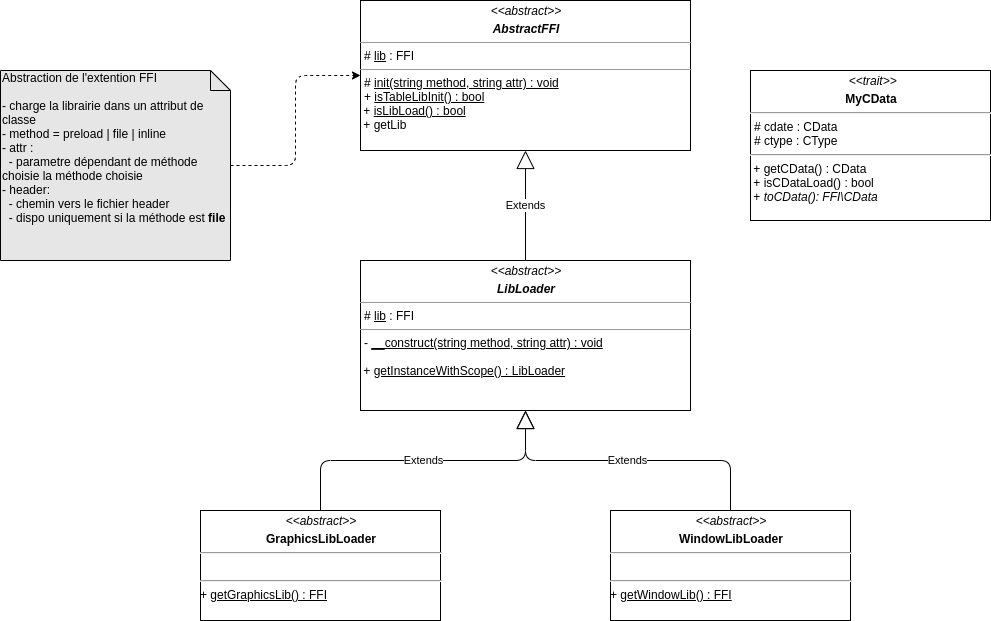
\includegraphics[width=0.9\linewidth]{assets/img/class-ffi-abstraction} 

}

\caption{Diagramme de classe : AbstractFFI}\label{fig:class-diagram-abstract-ffi}
\end{figure}

On y voit plusieurs classes abstraites, la principale étant \texttt{AbstractFFI} dont hérite \texttt{LibLoader}, leurs rôles est dans leur nom :

\begin{itemize}
\tightlist
\item
  \textbf{AbstractFFI} : la principale classe qui se charge de s'abstraire du chargement de la bibliothèque et de faire les vérifications nécessaires. Elle a comme attribut un tableau d'objets FFI pour permettre l'utilisation de plusieurs bibliothèques tout au long du programme.
\item
  \textbf{LibLoader} : héritant de AbstractFFI elle a les mêmes fonctionnalités, mais donne en plus la base pour mettre en place un \emph{singleton} de génération de bibliothèque --- une classe limité à une instance dont le seul objectif est de retourner une bibliothèque précise.
\end{itemize}

Pour ce qui est de \textbf{MyCData}, il s'agit d'un \texttt{trait}, particularité de PHP, qui est pour faire simple une classe abstraite qui s'utilise comme une interface. Son objectif est d'avoir un ensemble de fonctions et d'attributs prêts à être réutilisé pour définir une donnée C qui serait importée de la bibliothèque chargée avec FFI.

\hypertarget{architecture-globale}{%
\subsection{Architecture globale}\label{architecture-globale}}

Le reste de la bibliothèque est un ensemble de classes inspirées de SFML qui s'emboîtent autour de l'abstraction FFI. Effectivement, \textbf{SFML} et pas \textbf{C}SFML comme dit précédemment, car CSFML est juste un pont écrit en C vers SFML, or le C n'est pas un langage orienté objet. Par conséquent SFML qui est écrit en C++ qui lui est bien un langage orienté objet est idéal pour de servir de bases pour l'implémentation de mes classes. Toujours est-il que j'ai du simplifier un maximum l'architecture pour ne pas alourdir la bibliothèque en elle même et son utilisation finale.

\hypertarget{exemple-de-la-classe-window}{%
\subsection{Exemple de la classe Window}\label{exemple-de-la-classe-window}}

La classe Window est le deuxième pilier de l'architecture de la bibliothèque, comme la plupart des classes elle utilise MyCData pour bénéficier des méthodes et des attributs lier à l'échange de données entre PHP et la bibliothèque C via FFI. C'est le cas de la méthode \texttt{toCData()} qui convertit les attributs actuel de la classe en donnée C.

\hypertarget{diagramme-de-classes}{%
\subsection{Diagramme de classes}\label{diagramme-de-classes}}

Le résultat de la phase de conception est le diagramme de classe suivant qui a constamment évolué même lors de l'implémentation des fonctionnalités de la bibliothèque.

\label{fig:class-diagramm}\emph{Diagramme de classes intéractif accessible à l'adresse} \url{https://cutt.ly/phpml-class-diagram}

Le temps passé sur la réflexion de l'architecture de la bibliothèque n'a pas été en vain car il va nous permettre d'en gagner sur la partie principale qui est l'implémentation des fonctionnalités trouvées lors de la phase de conception.

\hypertarget{impluxe9mentation-de-la-bibliothuxe8que}{%
\section{Implémentation de la bibliothèque}\label{impluxe9mentation-de-la-bibliothuxe8que}}

L'implémentation des fonctionnalités se déroule lors de la phase de programmation, elle se déroule sans problèmes particuliers lorsque la phase de conception s'est bien déroulé car il n'y a pas besoin de réfléchir sur la structure de l'application ou de la bibliothèque car elle a déjà été définie. Néanmoins c'est au moment de l'implémentation qu'il faut penser à l'ordre de programmation des composants (bien que cela puisse être également fait lors de la conception) et que certaines faiblesses de conception apparaissent et je vais essayer d'en citer quelques unes.

\hypertarget{lordre-dimpluxe9mentation}{%
\subsection{L'ordre d'implémentation}\label{lordre-dimpluxe9mentation}}

Si la bibliothèque que l'on souhaite créer a des dépendances il est également probable que les éléments internes soient également interdépendants, cependant il est important de garder le niveau de dépendance le plus bas possible. C'est là que se pose la question de l'ordre l'implémentation. En ce qui me concerne j'ai préféré commencer par la classe principale et redescendre l'arbre de dépendance, ce qui n'est pas forcément la meilleure des solutions mais elle a eu le mérite d'être efficace et de me révéler certaines erreurs de conceptions que j'avais commises.

\hypertarget{erreurs-de-conception}{%
\subsection{Erreurs de conception}\label{erreurs-de-conception}}

La plus grande erreur que j'ai pu faire a été au niveau de l'abstraction, car j'utilisais un \texttt{trait} qui n'était pas vraiment adapté à ce que je concevais à la base, erreur qui m'a été notifié par ma tutrice de projet après consultation. En corrigeant cela j'ai pu aboutir à la version que vous pouvez voir au \ref{fig:class-diagram-abstract-ffi}.

En plus de diverses erreurs de conception corrigées sur le vif, j'ai été régulièrement confrontés à des erreurs de programmation plus techniques lié soit à FFI soit à CSFML. Celle qui m'a pris le plus de reflexions et de temps à corriger était une erreur de segmentation.

\begin{quote}
Une erreur de segmentation (en anglais segmentation fault, en abrégé segfault) est un plantage d'une application qui a tenté d'accéder à un emplacement mémoire qui ne lui était pas alloué.

\VA{--- \citep{wikipedia_segfault_2020}}{}
\end{quote}

Il faut également noter que je n'ai jamais été confronté à cette erreur \emph{en PHP} et il est très contraignant de retrouver la trace d'une erreur de segmentation quand on est développeur junior. Finalement il s'est avéré que retirer l'utilisation de la méthode \texttt{var\_dump()} de mon script résolvait mon erreur.

Une fois l'implémentation finis il faut à présent s'attarder à la distribution de notre bibliothèque.

\hypertarget{distribution-de-la-bibliothuxe8que}{%
\section{Distribution de la bibliothèque}\label{distribution-de-la-bibliothuxe8que}}

Cette section est purement subjective car il s'agit de choisir comment partager la version finale de la bibliothèque. Evidemment chacun peut avoir son avis, je vais donc plus m'intéresser au \emph{``comment''} plutôt qu'au \emph{``pourquoi''} j'ai choisi cette méthode.

\hypertarget{un-gestionnaire-de-paquets-composer}{%
\subsection{Un gestionnaire de paquets : composer}\label{un-gestionnaire-de-paquets-composer}}

\begin{quote}
Composer est un logiciel gestionnaire de dépendances libre écrit en PHP. Il permet à ses utilisateurs de déclarer et d'installer les bibliothèques dont le projet principal a besoin.

\VA{--- \citep{wikipedia_composer_2020}}{}
\end{quote}

\hypertarget{install-composer}{%
\subsection{Installation de composer}\label{install-composer}}

Pour installer composer nous avons juste besoin d'avoir php installé sur sa machine, ensuite les étapes d'installation sont détaillées sur la page d'\href{https://getcomposer.org/doc/00-intro.md\#installation-linux-unix-macos}{introduction à composer}. Mais pour résumer l'une des méthodes d'installation pour avoir composer globalement sur linux :

\begin{itemize}
\tightlist
\item
  Exécuter ces commandes pour télécharger la dernière archive de composer.
\end{itemize}

\begin{Shaded}
\begin{Highlighting}[]
\ExtensionTok{php}\NormalTok{ -r }\StringTok{"copy('https://getcomposer.org/installer', 'composer-setup.php');"}
\ExtensionTok{php}\NormalTok{ -r }\StringTok{"if (hash_file('sha384', 'composer-setup.php') === 'e0012edf3e80b6978849f5eff0d4b4e4c79ff1609dd1e613307e16318854d24ae64f26d17af3ef0bf7cfb710ca74755a') \{ echo 'Installer verified'; \} else \{ echo 'Installer corrupt'; unlink('composer-setup.php'); \} echo PHP_EOL;"}
\ExtensionTok{php}\NormalTok{ composer-setup.php}
\ExtensionTok{php}\NormalTok{ -r }\StringTok{"unlink('composer-setup.php');"}
\end{Highlighting}
\end{Shaded}

\begin{itemize}
\tightlist
\item
  Déplacer l'archive téléchargée vers son dossier bin :
\end{itemize}

\begin{Shaded}
\begin{Highlighting}[]
\FunctionTok{mv}\NormalTok{ composer.phar /usr/local/bin/composer}
\end{Highlighting}
\end{Shaded}

Avec composer installé nous pouvons créer intéractivement un fichier\texttt{composer.json} dans n'importe quel dossier ou projet avec la commande \texttt{composer\ init}.

\hypertarget{publication-de-bibliothuxe8que-avec-composer-et-packagist}{%
\subsection{Publication de bibliothèque avec composer et packagist}\label{publication-de-bibliothuxe8que-avec-composer-et-packagist}}

Avec composer il est facile de gérer les dépendances de son projet et de publier ses propres packets/bibliothèques. Les différentes étapes pour faire l'un ou l'autre sont brièvement décrites sur \href{https://packagist.org/}{packagist.org}. Pour faire court il est nécessaire d'avoir :

\begin{itemize}
\tightlist
\item
  un compte un \href{https://packagist.org/}{packagist.org}
\item
  un dépôt GIT
\item
  un fichier \texttt{composer.json} minimal à la racine de son dépôt :
\end{itemize}

\begin{Shaded}
\begin{Highlighting}[]
\FunctionTok{\{}
    \DataTypeTok{"name"}\FunctionTok{:} \StringTok{"vendor-name/package-name"}\FunctionTok{,}
    \DataTypeTok{"description"}\FunctionTok{:} \StringTok{"A short description of what your package does"}\FunctionTok{,}
    \DataTypeTok{"require"}\FunctionTok{:} \FunctionTok{\{}
        \DataTypeTok{"php"}\FunctionTok{:} \StringTok{"^7.2"}\FunctionTok{,}
        \DataTypeTok{"another-vendor/package"}\FunctionTok{:} \StringTok{"1.*"}
    \FunctionTok{\}}
\FunctionTok{\}}
\end{Highlighting}
\end{Shaded}

\hypertarget{maintenabilituxe9}{%
\subsection{Maintenabilité}\label{maintenabilituxe9}}

Une fois son packet ou sa bibliothèque publié sur packagist il est désormais possible à n'importe qui de ``demander'' votre bibliothèque via composer avec la commande \texttt{composer\ require\ vendor-name/package-name} à condition d'avoir également un fichier \texttt{composer.json} à la racine de son projet.

Ce qu'il nous reste à faire est de maintenir la bibliothèques, c'est à dire :

\begin{itemize}
\tightlist
\item
  aux nouvelles pratiques de notre langage et mises à jour de nos dépendances
\item
  ajouter de nouvelles fonctionnalités si on le souhaite.
\item
  re-publier sur packagist quand cela est fait (ou activer la mise à jour automatique sur son compte).
\end{itemize}

Nous avons donc terminé le développement y compris la distribution de notre bibliothèque, nous pouvons à présent apprendre à l'utiliser, ce qui n'est pas aussi trivial que nous pourrions le croire.

\hypertarget{tableau-ruxe9capitulatif}{%
\section{Tableau récapitulatif}\label{tableau-ruxe9capitulatif}}

\begin{longtable}[]{@{}ll@{}}
\caption{\label{tab:recap-dep} Récapitulatif des dépendances}\tabularnewline
\toprule
Dépendances & Commandes\tabularnewline
\midrule
\endfirsthead
\toprule
Dépendances & Commandes\tabularnewline
\midrule
\endhead
PHP 7.4 & \texttt{sudo\ apt\ install\ php7.4}\tabularnewline
FFI & \texttt{sudo\ apt\ install\ libffi-dev}\tabularnewline
SFML & \texttt{sudo\ apt\ install\ libsfml-dev}\tabularnewline
CSFML & \texttt{sudo\ apt\ install\ libcsfml-dev}\tabularnewline
Composer & voir le lien \url{https://getcomposer.org/download/}\tabularnewline
\bottomrule
\end{longtable}

\hypertarget{utils}{%
\chapter{Utilisation de la bibliothèque}\label{utils}}

\hypertarget{utils-pre-requis}{%
\section{Pré-requis à l'utilisation}\label{utils-pre-requis}}

Nous avons vu dans le \ref{pre-requis} que la bibliothèque développée comportait certaines dépendances résumé dans le \ref{tab:recap-dep}, PHP FFI et CSFML. Après les avoir installées il reste un minimum de configuration pour pouvoir parfaitement exécuter votre premier script.

\hypertarget{pruxe9chargement-ffi-et-header-csfml}{%
\subsection{Préchargement FFI et header CSFML}\label{pruxe9chargement-ffi-et-header-csfml}}

La bibliothèque utilise la fonctionnalité de préchargement de PHP pour précharger les header CSFML nécessaire pour charger et utiliser cette dernière en PHP. Il s'agit donc de modifier certaines variables de configuration de \texttt{php.ini} pour convenir à nos besoins. \emph{Les instructions données seront pour linux, il est possible que la procédure change sur windows}

\hypertarget{activation-de-ffi}{%
\subsubsection{Activation de FFI :}\label{activation-de-ffi}}

Il faut s'assurer que FFI est en mode \texttt{preload} et est bien activé

\begin{enumerate}
\def\labelenumi{\arabic{enumi}.}
\item
  dans le \texttt{php.ini} il faut que cette ligne soit présente \texttt{ffi.enable="preload"}
\item
  on peut vérifier la bonne activation de FFI avec la commande \texttt{php\ -m\ \textbar{}\ grep\ FFI} qui doit afficher \texttt{FFI}
\item
  activer \textbf{opcache} en ligne de commande en modifiant la valeur du paramètre \texttt{opcache.enable\_cli} à \texttt{true}.
\end{enumerate}

\hypertarget{mettre-en-place-le-pruxe9chargement}{%
\subsubsection{Mettre en place le préchargement :}\label{mettre-en-place-le-pruxe9chargement}}

Les fichiers header (extension en \texttt{.h}) à précharger sont dans le dossier \texttt{preloading} du dépot de la bibliothèque. Les deux premières ligne de chaque fichiers définissent :

\begin{itemize}
\tightlist
\item
  l'espace de définition utilisé pour charger la bibliothèque C en PHP, \textbf{à ne pas modifier}
\item
  le chemin \emph{absolu} vers le fichier binaire de la bibliothèque à charger, CSFML pour notre cas.

  \begin{itemize}
  \tightlist
  \item
    Il faut bien s'assurer que ce chemin est le bon pour réussir le chargement de la bibliothèque avec FFI. On peut vérifier cela avec la commande \texttt{locate}. Par exemple pour le module Graphics de CSFML il faut exécuter la commande \texttt{locate\ libcsfml-graphics.so}.
  \item
    \textbf{Attention !} si \emph{SFML} n'est pas installé avec \emph{CSFML} la bibliothèque ne pourra pas se charger.
  \end{itemize}
\end{itemize}

Le chemin absolu vers le dossier contenant ces fichiers doit être renseigné dans la variable \texttt{ffi.preload} du fichier de configuration de PHP en \textbf{ligne de commande}, sur ma machine son chemins est \texttt{/etc/php/7.4/cli/php.ini}. Ce chemin doit ensuite être suffixé de \texttt{*.h} pour préciser que nous voulons tous les fichiers d'extension \texttt{.h} situé dans ce dossier.

\begin{itemize}
\tightlist
\item
  Par exemple si le chemin vers le dossier \texttt{preloading} du dépôt est \texttt{/home/user/phpml/preloading/} la nouvelle valeur de la variable sera : \texttt{ffi.preload="/home/user/phpml/preloading/*.h"}
\end{itemize}

Si tout s'est bien passé, avec cette nouvelle configuration on devrait être capable d'exécuter un script de test du dépôt sans erreurs dès qu'on l'aura installé dans un nouveau projet avec composer.

\hypertarget{installation-dans-un-nouveau-projet}{%
\subsection{Installation dans un nouveau projet}\label{installation-dans-un-nouveau-projet}}

Partant du contexte que vous commencez un nouveau projet appelé \emph{nice-stuff} et que vous vouliez y intégrer cette bibliothèque, les étapes que vous aurez à réaliser doivent comprendre :

\begin{itemize}
\tightlist
\item
  la création du dossier \texttt{nice\_stuff}
\item
  l'initialisation de votre fichier \texttt{composer.json} avec \texttt{composer\ init}, après l'avoir préalablement installé \ref{install-composer}
\item
  l'ajout de la bibliothèque \textbf{PHPML} en tant que dépendance à votre projet : \texttt{composer\ require\ djuhnix/phpml}
\item
  il est important de noter que vous aurez besoin de la fonction d'autochargement fournie par composer :

  \begin{itemize}
  \tightlist
  \item
    il vous suffit de mettre au début de votre script la ligne ajoutant le fichier \texttt{vendor/autoload.php}. Cette ligne pourrait ressembler à \texttt{require\_once("vendor/autoload.php")} mais veillez à ce que le chemin passé à la fonction soit relatif à l'emplacement de votre script.
  \end{itemize}
\end{itemize}

A présent vous êtes prêt à utiliser la bibliothèque PHPML dans votre projet, composer s'occupera de charger les différentes classes que vous appellerez.

\hypertarget{exemple-dutilisation-et-documentations}{%
\section{Exemple d'utilisation et documentations}\label{exemple-dutilisation-et-documentations}}

\hypertarget{utilisation}{%
\subsection{Utilisation}\label{utilisation}}

Vous pouvez trouver des exemples d'utilisation de la bibliothèque dans le dossier \texttt{tests/functionnal} du dépôt git. Mais voici comment réaliser certaines tâches avec PHPML.

\hypertarget{comment-ouvrir-une-fenuxeatre}{%
\subsubsection{Comment ouvrir une fenêtre}\label{comment-ouvrir-une-fenuxeatre}}

Il deux façons d'ouvrir une fenêtre, la première consiste à utiliser la classe de base \texttt{Window} et gérer par sois même les boucles qui permettent de garder la fenêtre ouverte et de gérer les événements, notamment la fermeture de la fenêtre pour éviter de démarrer une boucle infini.

\begin{Shaded}
\begin{Highlighting}[]
\KeywordTok{$window}\NormalTok{ = }\KeywordTok{new}\NormalTok{ Window}\OtherTok{(}
    \KeywordTok{new}\NormalTok{ VideoMode}\OtherTok{(}\DecValTok{400}\OtherTok{,} \DecValTok{400}\OtherTok{),}
    \StringTok{'Test Window Opening'}
\OtherTok{);}
\KeywordTok{$event}\NormalTok{ = }\KeywordTok{new}\NormalTok{ Event}\OtherTok{();}

\CommentTok{//Début de la boucle (tant que la fenêtre est ouverte)}
\KeywordTok{while} \OtherTok{(}\KeywordTok{$window}\NormalTok{->isOpen}\OtherTok{())}\NormalTok{ \{}
    
    \CommentTok{// Gestion des événements}
    \KeywordTok{while} \OtherTok{(}\KeywordTok{$window}\NormalTok{->pollEvent}\OtherTok{(}\KeywordTok{$event}\NormalTok{->toCData}\OtherTok{()))}\NormalTok{ \{}
        \CommentTok{// Ferme la fenêtre si l'événement 'closed' est enregistré}
        \KeywordTok{if} \OtherTok{(}\KeywordTok{$event}\NormalTok{->}\FunctionTok{getType}\OtherTok{()}\NormalTok{->getValue}\OtherTok{()}\NormalTok{ == EventType::}\KeywordTok{CLOSED}\OtherTok{)}\NormalTok{ \{}
            \KeywordTok{$window}\NormalTok{->close}\OtherTok{();}
\NormalTok{        \}}
\NormalTok{    \}}
    
    \CommentTok{// DESSINER ICI}
    
    
    \CommentTok{// Nettoyage de l'écran de la fenêtre et affichage}
    \KeywordTok{$window}\NormalTok{->clear}\OtherTok{(}\KeywordTok{$window}\NormalTok{->getBackgroundColor}\OtherTok{());}
    
    \CommentTok{// rafraîchissement et affichage des dessins s'il y en a}
    \KeywordTok{$window}\NormalTok{->display}\OtherTok{();}
\NormalTok{\}}
\end{Highlighting}
\end{Shaded}

La création d'une instance de la classe \texttt{Window} nécessite obligatoirement de définir un mode de rendu qui contient également la taille de la fenêtre. Pour simplifier, la création de la fenêtre j'ai pris la décision de ne pas permettre la surcharge du mode de rendu vidéo et j'utilise celui de l'ordinateur par défaut, généralement de 32 bits par pixel.

Malgré cela, cette procédure restant fastidieuse à réaliser à chacun de ses scripts j'ai pensé à réaliser une autre classe \texttt{ExtendedWindow} héritant de la classe \texttt{Window} et qui étend ou plutôt facilite l'utilisation des fonctionnalités de cette dernière.

Désormais ouvrir une fenêtre revient à écrire

\begin{Shaded}
\begin{Highlighting}[]
\KeywordTok{$window}\NormalTok{ = }\KeywordTok{new}\NormalTok{ ExtendedWindow}\OtherTok{(}
    \KeywordTok{new}\NormalTok{ VideoMode}\OtherTok{(}\DecValTok{800}\OtherTok{,} \DecValTok{600}\OtherTok{)}
\OtherTok{);}

\KeywordTok{$window}\NormalTok{->run}\OtherTok{(}\KeywordTok{new}\NormalTok{ Event}\OtherTok{());}
\end{Highlighting}
\end{Shaded}

Comme le dit la documentation, la méthode \texttt{run()} de la classe \texttt{Window}

\begin{quote}
Lance la boucle principale de la fenêtre et l'ouvre dans le même temps.
\end{quote}

En plus de cela elle gère également la boucle d'événement qui s'occupe de la fermeture de la fenêtre, s'occupe de dessiner à chaque rafraîchissement les objets qui lui sont attachés et possède bien plus d'atouts que nous détaillerons plus tard. Cette méthode facilite l'utilisation de bibliothèque à un point considérable car elle permet de s'abstraire des tâches répétitives lié à la création d'une fenêtre dans les bibliothèques graphiques classiques, c'est également la pierre angulaire de la librairie parce que c'est par elle que commence toutes activités que l'on voudrait réaliser avec la bibliothèque, comme dessiner des formes.

\hypertarget{comment-dessiner}{%
\subsubsection{Comment dessiner}\label{comment-dessiner}}

Pour dessiner sur une fenêtre il n'y a rien de plus simple que l'appelle à la méthode \texttt{draw()} de la classe \texttt{Window} qui prend en paramètre un objet ``dessinable'' préalablement initialisé (de préférence à l'extérieur de la boucle) et l'affiche sur la fenêtre actuelle.

Après avoir ouvert notre fenêtre, en supposant qu'on utilise la première méthode qu'offre notre bibliothèque, il faudrait écrire dans la partie réserver aux dessins (mise en évidence plus haut) :

\begin{Shaded}
\begin{Highlighting}[]
\KeywordTok{$window}\NormalTok{->draw}\OtherTok{(}
            \KeywordTok{new}\NormalTok{ RectangleShape}\OtherTok{(}
                \OtherTok{[}\DecValTok{400}\OtherTok{,} \DecValTok{200}\OtherTok{],}
                \OtherTok{[}\DecValTok{100}\OtherTok{,} \DecValTok{200}\OtherTok{],}
                \KeywordTok{$blue}
            \OtherTok{)}
        \OtherTok{);}
\end{Highlighting}
\end{Shaded}

Cependant faire cela est une mauvaise pratique et il serait préférable de créer ses formes avant le lancement de la boucle de la fenêtre, cela empêcherait l'inutile création de la même forme tout au long de la boucle qui maintient la fenêtre ouverte.

Cela reste valable même si l'on utilise la seconde possibilité d'ouverture de fenêtre qu'est la méthode \texttt{run()} de la \texttt{ExtendedWindow}. Pour revenir sur cette méthode, il faut savoir qu'elle prend en paramètre en plus de la variable d'événements, deux fonctions qui sont respectivement utilisé pour la gestion personnalisée d'événements par l'utilisateur et la réalisation de dessins sur la fenêtre, s'il n'y a que cette dernière option qui nous intéresse on peut toujours passé null à la fonction \texttt{run()} à la place de la fonction de gestion d'événements. Il est vrai que cette façon de faire nécessite de connaître le concept de fonction anonyme (closure) qui relève de l'algorithmie légèrement avancé pour un débutant mais dès qu'on sait comment l'utiliser le reste n'est que de simples détails théoriques.

\begin{Shaded}
\begin{Highlighting}[]
\KeywordTok{$text}\NormalTok{ = }\KeywordTok{new}\NormalTok{ Text}\OtherTok{(}\StringTok{"Hello"}\OtherTok{);}
\KeywordTok{$text}\NormalTok{->setFillColor}\OtherTok{(}\KeywordTok{$blue}\OtherTok{);}
\KeywordTok{$text}\NormalTok{->setPosition}\OtherTok{([}\DecValTok{150}\OtherTok{,} \DecValTok{50}\OtherTok{]);}
\KeywordTok{$text}\NormalTok{->setCharacterSize}\OtherTok{(}\DecValTok{50}\OtherTok{);}

\KeywordTok{$window}\NormalTok{->run}\OtherTok{(}
    \KeywordTok{new}\NormalTok{ Event}\OtherTok{(),}
    \KeywordTok{null}\OtherTok{,}
    \KeywordTok{function} \OtherTok{()} \KeywordTok{use} \OtherTok{(}\KeywordTok{$text}\OtherTok{,} \KeywordTok{$window}\OtherTok{)}\NormalTok{ \{}
        \KeywordTok{$window}\NormalTok{->draw}\OtherTok{(}\KeywordTok{$text}\OtherTok{);}
\NormalTok{    \}}
\OtherTok{);}
\end{Highlighting}
\end{Shaded}

Le mot clé use est là pour dire que nous voulons utiliser ces variables pré-définie à l'interieur de notre fonction anonyme, sinon PHP ne sait pas que ces variables ont bien été déclaré et initialisé. Notre fonction anonyme peut ne pas être si anonyme qu'on peut le croire car on peut lui donner un nom, l'enregistrer dans une variable et passer cette dernière dans à la méthode \texttt{run()} plus tard dans notre script.

\begin{Shaded}
\begin{Highlighting}[]
\KeywordTok{function}\NormalTok{ dessine}\OtherTok{()}\NormalTok{ \{}
\StringTok{...}
\NormalTok{\}}

\KeywordTok{$maFonction}\NormalTok{ = }\StringTok{'dessine'}\OtherTok{;}
\CommentTok{//ou}
\KeywordTok{$maFonction}\NormalTok{ = }\KeywordTok{function} \OtherTok{()}\NormalTok{ \{}
\StringTok{...}
\NormalTok{\}}

\KeywordTok{$window}\NormalTok{->run}\OtherTok{(}\KeywordTok{new}\NormalTok{ Event}\OtherTok{(),} \KeywordTok{null}\OtherTok{,} \KeywordTok{$maFonction}\OtherTok{);}
\end{Highlighting}
\end{Shaded}

Cependant il faut prendre en compte le fait que si l'on utiliser des variables mise à jour dynamiquement par la bibliothèque comme les événements cette méthode est à proscrire.

\hypertarget{comment-garder-les-modifications-appliquuxe9es-uxe0-ses-objets}{%
\subsubsection{Comment garder les modifications appliquées à ses objets}\label{comment-garder-les-modifications-appliquuxe9es-uxe0-ses-objets}}

Par défaut la bibliothèque n'enregistre pas toutes les modifications que vous appliquer à vos formes et autres objets dessinables parce qu'ils ne sont pas attachés à la fenêtre. Pour ce faire il faut utiliser la méthode \texttt{addToDrawingList()} qui comme son nom l'indique ajoute un objet identifié par une clé à la liste des éléments à dessiner qui seront enregistrés avec les données de la fenêtre et mis à jour à toutes futures modifications. L'objet enregistré peut toujours être retrouvé grâce à son identifiant et modifié si besoin.

\begin{Shaded}
\begin{Highlighting}[]
\KeywordTok{$window}\NormalTok{->addToDrawingList}\OtherTok{(}
    \StringTok{'rectangle'}\OtherTok{,} \CommentTok{// la clé de l'objet}
    \KeywordTok{new}\NormalTok{ RectangleShape}\OtherTok{(}
        \OtherTok{[}\DecValTok{400}\OtherTok{,} \DecValTok{200}\OtherTok{],}
        \OtherTok{[}\DecValTok{100}\OtherTok{,} \DecValTok{200}\OtherTok{],}
        \KeywordTok{new}\NormalTok{ Color}\OtherTok{(}\NormalTok{Color::}\KeywordTok{BLUE}\OtherTok{)} \CommentTok{// définition de la couleur de fond en bleue}
    \OtherTok{)}
\OtherTok{);}

\KeywordTok{$window}\NormalTok{->run}\OtherTok{(}
    \KeywordTok{new}\NormalTok{ Event}\OtherTok{(),}
    \KeywordTok{null}\OtherTok{,}
    \KeywordTok{function} \OtherTok{()} \KeywordTok{use} \OtherTok{(}\KeywordTok{$red}\OtherTok{,} \KeywordTok{$window}\OtherTok{)}\NormalTok{ \{}

        \KeywordTok{$window}
\NormalTok{            ->getDrawingList}\OtherTok{()}
\NormalTok{            ->getObject}\OtherTok{(}\StringTok{'rectangle'}\OtherTok{)}
\NormalTok{            ->setFillColor}\OtherTok{(}\KeywordTok{$red}\OtherTok{)} \CommentTok{// Le rectangle affiché sera rouge au lieu d'être bleue comme défini plus haut}
    \OtherTok{;}
\NormalTok{    \}}
\OtherTok{);}
\end{Highlighting}
\end{Shaded}

Tout cela dans le but de faciliter l'utilisation de la bibliothèque par des débutants et surtout flexibilité de celle-ci.

\hypertarget{extra}{%
\subsubsection{Extra}\label{extra}}

\hypertarget{cruxe9er-une-couleur}{%
\paragraph{Créer une couleur}\label{cruxe9er-une-couleur}}

Des couleurs sont prédéfinie dans l'énumération prévu pour. Mais pour s'en servir il faut créer une instance de couleur avec l'une de ces valeurs.

\begin{Shaded}
\begin{Highlighting}[]
\KeywordTok{$color}\NormalTok{ = }\KeywordTok{new}\NormalTok{ Color}\OtherTok{(}\NormalTok{Color::}\KeywordTok{RED}\OtherTok{)} \CommentTok{// équivaut à Color::DYNAMIC()}
\end{Highlighting}
\end{Shaded}

Il est évidemment possible de créer des couleurs dynamique avec des valeur de couleurs primaires.

\begin{Shaded}
\begin{Highlighting}[]
\KeywordTok{$color}\NormalTok{ = }\OtherTok{(}\KeywordTok{new}\NormalTok{ Color}\OtherTok{(}\NormalTok{Color::}\KeywordTok{DYNAMIC}\OtherTok{))} \CommentTok{// équivaut à Color::DYNAMIC()}
\NormalTok{    ->fromRGB}\OtherTok{(}\DecValTok{12}\OtherTok{,} \DecValTok{12}\OtherTok{,} \DecValTok{13}\OtherTok{);}
\end{Highlighting}
\end{Shaded}

\hypertarget{guxe9rer-des-uxe9vuxe9nements}{%
\paragraph{Gérer des événements}\label{guxe9rer-des-uxe9vuxe9nements}}

On ne pourrait pas parler proprement de bibliothèque graphique sans gestion des événements déclencher sur la fenêtre, voilà pourquoi l'implémentation de la gestion des événements et des entrées (clavier et souris) faisaient parties de mes priorités.

On a précédemment vu sur les morceaux de codes qu'on pouvait créer une instance d'événement avec

\begin{Shaded}
\begin{Highlighting}[]
\KeywordTok{new}\NormalTok{ Event}\OtherTok{()}
\end{Highlighting}
\end{Shaded}

Le constructeur de cette classe ne prend rien en paramètre car tout est géré en interne pour l'utilisateur. Tout ce qu'il reste à faire pour l'utiliser c'est de vérifier qu'un certain type d'événement à bien été reçu et le traiter en tant que tel. Un exemple d'utilisation serait :

\begin{Shaded}
\begin{Highlighting}[]
\KeywordTok{$event}\NormalTok{ = }\KeywordTok{new}\NormalTok{ Event}\OtherTok{();}
\KeywordTok{$window}\NormalTok{->run}\OtherTok{(}
    \KeywordTok{$event}\OtherTok{,}
    \KeywordTok{function} \OtherTok{()} \KeywordTok{use} \OtherTok{(}\KeywordTok{$event}\OtherTok{,} \KeywordTok{$window}\OtherTok{)}\NormalTok{ \{}
        \KeywordTok{if} \OtherTok{(}\KeywordTok{$event}\NormalTok{->}\FunctionTok{getType}\OtherTok{()}\NormalTok{->getValue}\OtherTok{()}\NormalTok{ == EventType::}\KeywordTok{MOUSE_BUTTON_PRESSED}\OtherTok{)}\NormalTok{ \{}
            \CommentTok{// réaliser une action si un bouton de la souris est cliqué}
\NormalTok{        \}}
\NormalTok{    \}}\OtherTok{,}
    \KeywordTok{function} \OtherTok{()} \KeywordTok{use} \OtherTok{(}\KeywordTok{$event}\OtherTok{,} \KeywordTok{$window}\OtherTok{)}\NormalTok{ \{}
       \CommentTok{// faire ses dessins}
\OtherTok{);}
\end{Highlighting}
\end{Shaded}

\hypertarget{documentation}{%
\subsection{Documentation}\label{documentation}}

Actuellement la documentation de la bibliothèque n'est pas hébergé mais elle peut être lu directement sur les sources de la bibliothèque sur le dépôt github.

\hypertarget{res}{%
\chapter{Résultat}\label{res}}

\hypertarget{finalituxe9-de-la-bibliothuxe8que}{%
\section{Finalité de la bibliothèque}\label{finalituxe9-de-la-bibliothuxe8que}}

A la fin de mes quatre semaines de travail j'ai pu implémenté la majorité sinon toutes les fonctionnalités demandées par ma tutrice de projets pour cette mise en situation professionnelle. On peut alors être fier et dire que l'objectif est atteint, malgré tout la bibliothèque n'est pas complète et il reste des choses à approfondir.

Par exemple la possibilité de créer des formes personnalisé en redéfinissant ou en héritant de la classe \texttt{Shape} comme cela est expliqué dans un tutoriel de SFML sur \href{https://www.sfml-dev.org/tutorials/2.5/graphics-shape-fr.php\#formes-personnaliscees}{la création de forme}. C'est l'une des choses que j'aurai aimé implémenter sur la fin de ma période de travail avec la création de formes convexes --- la classe \href{https://www.sfml-dev.org/documentation/2.5.1-fr/classsf_1_1ConvexShape.php}{\texttt{ConvexShape}}. Ce qui ne pourra pas être fait par manque de temps mais surtout de capacités offertes par FFI.

Le principal étant que la bibliothèque soit utilisable pour les TPs de POO, l'implémentation de ce genre de fonctionnalités complexes passe au second plan. Même si cela n'est pas impossible, il est peut probable qu'un débutant puisse avoir l'initiative de se lancer dans ce genre de défi.

\hypertarget{bilan-de-la-mise-en-situation-professionnelle}{%
\section{Bilan de la mise en situation professionnelle}\label{bilan-de-la-mise-en-situation-professionnelle}}

La mise en situation professionnelle fut une épreuve très enrichissante sur tellement de points que je ne pourrai tous les aborder.

Elle m'a d'abord aidé à développer des compétences nouvelles tout comme à approfondir et étendre celles que je possédais déjà. Je pourrai citer la découverte et l'utilisation maximale des nouveautés qu'apporte le PHP 7.4 dans la création de PHPML mais aussi la connaissance du C --- que je n'ai jamais pratiqué --- et la bibliothèque SFML. Elle a également permis la culture de bonnes habitudes personnelle et professionnel grâce à la confrontation au télétravail, ce qui n'aurait pas forcément été possible lors d'un stage.

Il est certains que créer un package PHP n'est pas un projet aisé qui se fait dès la première idée. J'ai donc du établir un plan de développement et l'adapter à chaque évolution du projet que ce soit sur la conception ou l'implémentation, cela à évidemment contribuer à élargir la vision que j'avais de la gestion de projet et dans le même temps améliorer mes compétences dans le domaine.

Pourtant il est difficile de croire que la mise ne situation professionnelle n'a que des qualités. En effet, malgré tout ce que j'ai gagné à réaliser ce projet il ne sera pas officiellement compté comme une expérience professionnelle; la où mon stage aurait permis d'en avoir un minimum et me démarquer parmi tous les autres débouchés la mise en situation professionnelle n'est qu'un projet de plus dans mon cursus d'étudiants.

\hypertarget{ressenti-personnel}{%
\section{Ressenti personnel}\label{ressenti-personnel}}

Globalement j'ai un ressenti positif envers l'expérience que j'ai vécu lors de ma mise en situation professionnelle. Il est plus pertinent de se faire un point de vue sur les bénéfices que sur les inconvénients.

Il était éprouvant psychologiquement de travailler au même endroit ou je me divertis, se retenir d'arrêter le travail pour jouer par exemple, alors que presque tout était réuni pour, fut l'un des efforts que j'ai du fournir pour arriver au terme du projet ou du moins à un minimum viable.

J'ai été confronté à divers problématiques que je n'ai pas tout le temps réussi à résoudre ou que j'ai failli abandonner, mais quoiqu'il en était contourner le problème pour y arriver ou demander conseil à ma tutrice de projet a toujours été le meilleur choix. Finalement j'en suis sorti avec plus d'acquis qu'avant et c'est je pense le plus important. \^{}

\hypertarget{conclusion}{%
\chapter*{Conclusion}\label{conclusion}}


Pour décharger les tâches des professeurs du département informatique de l'IUT de Reims, liées à l'enseignement de la POO, il a été décidé de réaliser une bibliothèque graphique Java. Cependant elle a du être abandonné à cause du changement de langage dans le nouveau programme. Le projet de construire une nouvelle bibliothèque en PHP m'a donc été confié pour ma mise en situation professionnelle.

Le but était alors de trouver comment créer une bibliothèque orientée objets en PHP avec les mêmes possibilités que celle précédemment utilisé par le département, la principale étant l'ouverture d'une fenêtre système et le dessin de formes sur cette fenêtre à l'aide de manipulations et d'instanciations d'objets. Tout en considérant le fait que ce sujet n'avait pas encore été abordé en profondeur pour avoir une base de travail et que de plus je n'en avait aucune connaissance jusqu'à ce que je plonge dans la phase de recherches.

Avec les pointeurs que j'ai reçu en début de projet j'ai réussi grâce à FFI à implémenter une partie du module Graphics de CSFML en PHP et grâce à composer et packagist j'ai pu la distribuer pour une utilisation public. \textbf{PHPML} répond parfaitement aux réquisitions d'une bibliothèque PHP orientée objets et en ce qui concerne ses fonctionnalités elle comprend celles demandés en priorité par ma tutrice de projet. Bien que légère par rapport à toutes les fonctionnalités de l'ancienne bibliothèque et de CSFML elle pourra satisfaire les premiers besoins pour lesquels elle a été créer: alléger la création des travaux pratiques par les professeurs et leurs réalisations par les étudiants.

Ainsi j'ai pu apprendre à créer une bibliothèque en PHP et me servir de FFI, sans oublier la gestion de mon temps et de mon projets en télétravail. Néanmoins tout n'est pas accompli, le minimum pour la suite serait l'implémentation complète du module Graphics de CSFML pour mettre à jour cette librairie et l'apogée l'ajout de tous les modules composant CSFML pour que PHPML porte réellement son nom. Malgré la motivation éprouvé à l'égard de ce que serait cet exploit il ne sera pas aisé de réaliser notre volonté à ce jour étant donné les limitations actuelles de FFI et l'investissement de temps que cela représente. Mais on peut déjà espérer développer de petits projets avec ce qu'est PHPML aujourd'hui.

\hypertarget{liste-des-abbreviations}{%
\chapter*{Liste des Abbreviations}\label{liste-des-abbreviations}}


\begin{description}
\item[POO]
Programmation Orientée Objets

\begin{quote}
La programmation orientée objet (POO), ou programmation par objet, est un paradigme de programmation informatique. Il consiste en la définition et l'interaction de briques logicielles appelées objets ; un objet représente un concept, une idée ou toute entité du monde physique, comme une voiture, une personne ou encore une page d'un livre.
\end{quote}

--- \citep{wikipedia_programmation_2020}
\item[FFI]
Foreign Function Interface

C'est un mécanisme par lequel un programme écrit dans un langage de programmation peut appeler des routines ou utiliser des services écrits dans un autre.
\item[SFML]
Simple and Fast Media Library

\begin{quote}
SFML offre une interface simple vers les différents composants de votre PC, afin de faciliter le développement de jeux ou d'applications multimedia. Elle se compose de cinq modules : système, fenêtrage, graphisme, audio et réseau.
\end{quote}

--- \citep{laurent_sfml_2020}
\item[CSFML]
C Simple and Fast Media Library

\begin{quote}
CSFML est le binding officiel de SFML pour le langage C. Son API est aussi proche que possible que l'API C++ (mais dans le style C, bien entendu), ce qui en fait un candidat parfait pour construire des bindings SFML pour d'autres langages qui ne supportent pas directement les bibliothèques C++.
\end{quote}

--- \citep{laurent_sfml_2020}
\item[URCA]
Université de Reims Champagne Ardenne
\item[IUT-RCC]
Institut Universitaire de Technologie de Reims-Châlons-Charleville
\end{description}

\backmatter

\bibliography{bib/book.bib,bib/citations.bib,packages.bib}

\printindex

\end{document}
